% !TEX root = ../../../main.tex
% 来源：中学数学实验教材·第三册（高中数学）
% 章节：指数概念普遍化与对数 / 对数和常用对数
% 原始文件：1.tex，行 2667-2675
% 类型：tikz
% ---
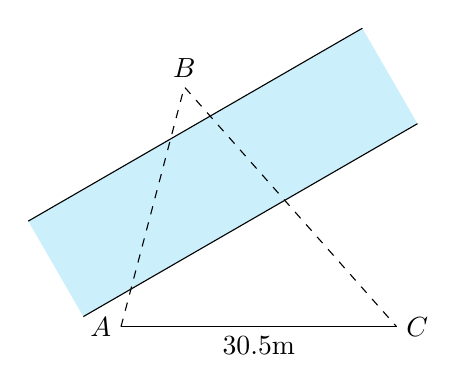
\begin{tikzpicture}[>=latex, scale=.7]
    \fill[rotate=30, cyan!20] (-.5,0.5) rectangle (6.5,2.5);
    \draw[rotate=30] (-.5,.5)--(6.5,.5)    ;
    \draw[rotate=30]  (-.5,2.5)--(6.5,2.5)    ;  
\draw[dashed] (0,0)node[left]{$A$}--(75.2:4.5)node[above]{$B$}--(5,0);
\draw (5,0)node[right]{$C$}--node[below]{30.5m}(0,0);


    \end{tikzpicture}
